\section{Fundamental group of the circle and applications}
03.04

\begin{theorem}
    For all \( x \in \mathbb{S}^1 \)
    we have that
    \[
      \pi_1(\mathbb{S}^1, x) \simeq \mathbb{Z}
    \] 
    is an isomorphism of groups.
\end{theorem}

\begin{proof}
    Since \( \mathbb{S}^1 \) is path connected
    it suffices to show the claim for some \( x_0 \in \mathbb{S}^1 \).
    Let \( x_0 = (1, 0) \).
    For the lifting correspondence, pick
    \( 0 \in \mathbb{R} \) and
    \( p: \mathbb{R} \to \mathbb{S}^1 \)
    sending
    \[
      p(t) = (\cos 2 \pi t, \sin 2 \pi t)
    \]
    By corollary \ref{cor:S1_Z_bij}
    we have a bijection, so we need to show
    that it is a group homomorphism.

    Let \( \gamma_1, \gamma_2: I \to \mathbb{S}^1 \) be paths.
    Let \( \tilde{\gamma}_1, \tilde{\gamma}_2 \) be
    the unique lifts. Let \[ \tilde{\gamma}_1(1) = n, \tilde{\gamma}_2(1) = m \]
    We need to show that \[ (\widetilde{\gamma_2 * \gamma_1})(1) = n + m \]
    We do this by constructing the lift of \( \gamma_2 * \gamma_1 \).
    Define \( h: I \to \mathbb{R} \) by
    \[
      h(s) = \tilde{\gamma}_2(s) + \tilde{\gamma}_1(1)
    \]
    Consider
    \[
      (h * \tilde{\gamma}_1)(s) = \begin{cases}
        \tilde{\gamma}_1(s) (2s) & 0 \le s \le 1/2 \\
        h(2s - 1) & 1/2 \le s \le 1
      \end{cases}
    \]
    \( h * \tilde{\gamma}_1 \) satisfies the
    property we want since
    \[
      (h * \tilde{\gamma}_1)(0) = \tilde{\gamma}_1(0) = 0
    \]
    and
    \[
      (h * \tilde{\gamma}_1)(1) = h(1)
      = \tilde{\gamma}_1(1) + \tilde{\gamma}_2(1)
      = n + m
    \]
    Let's verify that \( h * \tilde{\gamma}_1 \)
    is actually the lift of \( \gamma_2 * \gamma_1 \)
    by showing that
    \(
      p \circ (h * \tilde{\gamma}_1) = \gamma_2 * \gamma_1
    \).
    \begin{align*}
      (p \circ (h * \tilde{\gamma_1}))(s)
        &= \begin{cases}
          (p \circ \tilde{\gamma}_1) (2s) & 0 \le s \le 1/2 \\
          (p \circ h) (2s - 1) & 1/2 \le s \le 1
        \end{cases} \\
        &= \begin{cases}
          \gamma_1(2s) & 0 \le s \le 1/2 \\
          p\left(\tilde{\gamma}_1(1) + \tilde{\gamma}_2(2s - 1)\right) & 1/2 \le s \le 1
        \end{cases} \\
        &= \begin{cases}
          \gamma_1(2s)      & 0 \le s \le 1/2 \\
          \gamma_2(2s - 1)  & 1/2 \le s \le 1
        \end{cases} \\
        &= (\gamma_2 * \gamma_1)(s)
    \end{align*}
\end{proof}


\subsection{Applications of the fundamental group of the circle}

\begin{lemma}
  \label{lma:S1_not_retract_of_X}
    Let \( X \) be a space
    such that
    \( \pi_1(X, x) = * \).
    Suppose there exists a map
    \( f: \mathbb{S}^1 \to X \).
    Then \( \mathbb{S}^1 \) cannot
    be a retract of \( X \).
\end{lemma}

\begin{proof}
    Suppose a retract \( r: X \to \mathbb{S}^1 \) exists.
    Then we get:
      % https://q.uiver.app/#q=WzAsNixbMCwwLCJcXG1hdGhiYntTfV4xIl0sWzIsMCwiWCJdLFs0LDAsIlxcbWF0aGJie1N9XjEiXSxbMCwyLCJcXG1hdGhiYntafSJdLFsyLDIsIjAiXSxbNCwyLCJcXG1hdGhiYntafSJdLFswLDEsImYiXSxbMSwyLCJyIl0sWzAsMiwiXFx0ZXh0e2lkfSIsMCx7ImN1cnZlIjozfV0sWzMsNF0sWzQsNV0sWzMsNSwiXFx0ZXh0e2lkfSIsMCx7ImN1cnZlIjozfV0sWzgsNCwiXFxwaV8xIiwyLHsic2hvcnRlbiI6eyJzb3VyY2UiOjIwfX1dXQ==
  \[\begin{tikzcd}
    {\mathbb{S}^1} && X && {\mathbb{S}^1} \\
    \\
    {\mathbb{Z}} && 0 && {\mathbb{Z}}
    \arrow["f", from=1-1, to=1-3]
    \arrow[""{name=0, anchor=center, inner sep=0}, "{\text{id}}", curve={height=18pt}, from=1-1, to=1-5]
    \arrow["r", from=1-3, to=1-5]
    \arrow[from=3-1, to=3-3]
    \arrow["{\text{id}}", curve={height=18pt}, from=3-1, to=3-5]
    \arrow[from=3-3, to=3-5]
    \arrow["{\pi_1}"', shorten <=5pt, Rightarrow, from=0, to=3-3]
  \end{tikzcd}\]
  which is a contradiction since \( \text{id}: \mathbb{Z} \to \mathbb{Z} \)
  does not factor through \( 0 \).
\end{proof}

\begin{theorem}[Brouwer fixed point]
   Let \( D^2 := \{ (x, y) \in \mathbb{R}^2 \mid x^2 + y^2 \le 1 \}  \).
   Then given a continuous map
   \( f: D^2 \to D^2 \) there exists
   a point in the disk such that \( f(x) = x \).
\end{theorem}

\begin{proof}
    Suppose there exists a continuous map
    \[
      f: D^2 \to D^2
    \]
    without fixed points.
    Then there exists a retract
    \[
      r: D^2 \to \mathbb{S}^1
    \]
    defined by constructing the ray
    at \( x \) through \( f(x) \) and letting
    \( r(x)  \) be the intersection at \( \mathbb{S}^1 \).
    This is a contradiction by lemma \ref{lma:S1_not_retract_of_X}
    since \( D^2 \) is homotopy equivalent to a point.
    \begin{center}
    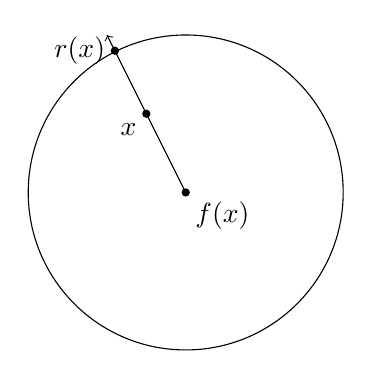
\begin{tikzpicture}
      \draw (0, 0) circle (2);
      \draw[->] (0, 0) to (-1, 2);
      \fill (0, 0) circle (1.5pt) node[below right] {$f(x)$};
      \fill (-0.5, 1) circle (1.5pt) node[below left] {$x$};
      \fill (-0.9, 1.8) circle (1.5pt) node[left] {$r(x)$};
    \end{tikzpicture}
  \end{center}
\end{proof}

\begin{lemma}
    Let \( h: \mathbb{S}^1 \to X \).
    Then \( h \) is nullhomotopic
    if
    \[
      \pi_1(h): \pi_1(\mathbb{S}^1, a) \to \pi_1(X, h(a))
    \]
    is the trivial map.
\end{lemma}

\begin{proof}
    My notes are not easy to read.
    See proof in Hatcher.
\end{proof}

\subsection{Study tips}
Pass (bare minimum):
\begin{enumerate}
  \item topological spaces, cont. maps
    \subitem interior, closure, metric spaces
  \item constructions with topological spaces
    \subitem subspaces
    \subitem products
    \subitem quotients
  \item properties of topological spaces
    \subitem Hausdorff
    \subitem compact
    \subitem connected
  \item which properties are stable under which constructions?
    \subitem find counterexamples, make a table
  \item homotopy theory
    \subitem homotopy
    \subitem path homotopy
    \subitem homotopy equivalence
    \subitem fundamental group
    \subitem \( \pi_1(\mathbb{S}^1) = \mathbb{Z} \)
    \subitem functoriality
\end{enumerate}

Bonus:
\begin{enumerate}
  \item which properties are stable under homotopy equivalence?
\end{enumerate}

